% ****** Start of file apssamp.tex ******
%
%   This file is part of the APS files in the REVTeX 4.1 distribution.
%   Version 4.1r of REVTeX, August 2010
%
%   Copyright (c) 2009, 2010 The American Physical Society.
%
%   See the REVTeX 4 README file for restrictions and more information.
%
% TeX'ing this file requires that you have AMS-LaTeX 2.0 installed
% as well as the rest of the prerequisites for REVTeX 4.1
%
% See the REVTeX 4 README file
% It also requires running BibTeX. The commands are as follows:
%
%  1)  latex apssamp.tex
%  2)  bibtex apssamp
%  3)  latex apssamp.tex
%  4)  latex apssamp.tex

\documentclass[
reprint,
%superscriptaddress,
%groupedaddress,
%unsortedaddress,
%runinaddress,
%frontmatterverbose,
%preprint,
showpacs,preprintnumbers,
%nofootinbib,
%nobibnotes,
%bibnotes,
amsmath,amssymb,
%aps,
prl,
%prb,
%rmp,
%prstab,
%prstper,
%floatfix,
]{revtex4-1}

\usepackage{graphicx} % Include figure files
\usepackage{dcolumn} % Align table columns on decimal point
\usepackage{bm} % bold math
\usepackage{hyperref} % add hypertext capabilities
%\usepackage[mathlines]{lineno}% Enable numbering of text and display math
%\linenumbers\relax % Commence numbering lines

%\usepackage[showframe,%Uncomment any one of the following lines to test
%%scale=0.7, marginratio={1:1, 2:3}, ignoreall,% default settings
%%text={7in,10in},centering,
%%margin=1.5in,
%%total={6.5in,8.75in}, top=1.2in, left=0.9in, includefoot,
%%height=10in,a5paper,hmargin={3cm,0.8in},
%]{geometry}

\begin{document}

\title{Animal Swarming} % Force line breaks with \\
\thanks{Simulation \& Theory}

\author{Jan Polivka (ID:51553399)}
 \email{j.polivka.15@aberdeen.ac.uk}
\author{Struan Murray (ID:51550442)}
 \email{struan.murray.15@aberdeen.ac.uk}
\author{Daniel Bain (ID:51443692)}
 \email{daniel.m.bain.14@aberdeen.ac.uk}
\affiliation{University of Aberdeen}

\date{\today}

\begin{abstract}
	\noindent{}Swarming of animals has been known to form complex patterns and this report covers the basic processes required to recreate these forms in a simulation as well as the theory and analysis of these swarms as a form of defense against predators.
\end{abstract}

\pacs{\href{https://ufn.ru/en/pacs/87.19.St/}{87.19.St}, \href{https://ufn.ru/en/pacs/all}{87.19.lp}}
\maketitle

%\tableofcontents

\section{\label{sec:level1}Introduction to Swarming}

The collective movement of animals can produce eye-catching patterns in a seemingly complex yet ordered fashion. (FIG. \ref{fig:birdswarm})
These patterns can hypothetically be assigned to the similar reactions of the individual animals in the presence of danger, prospect of food or safety.
Similar patterns of ``Swarming" have also recently been discovered in purely chemical reactions where individual units are self propelled.\cite{collectivemotion}
This suggests that a large proportion of the swarming behaviour may be as a result of very simple rules.

\begin{figure}[!htp]
	\fbox{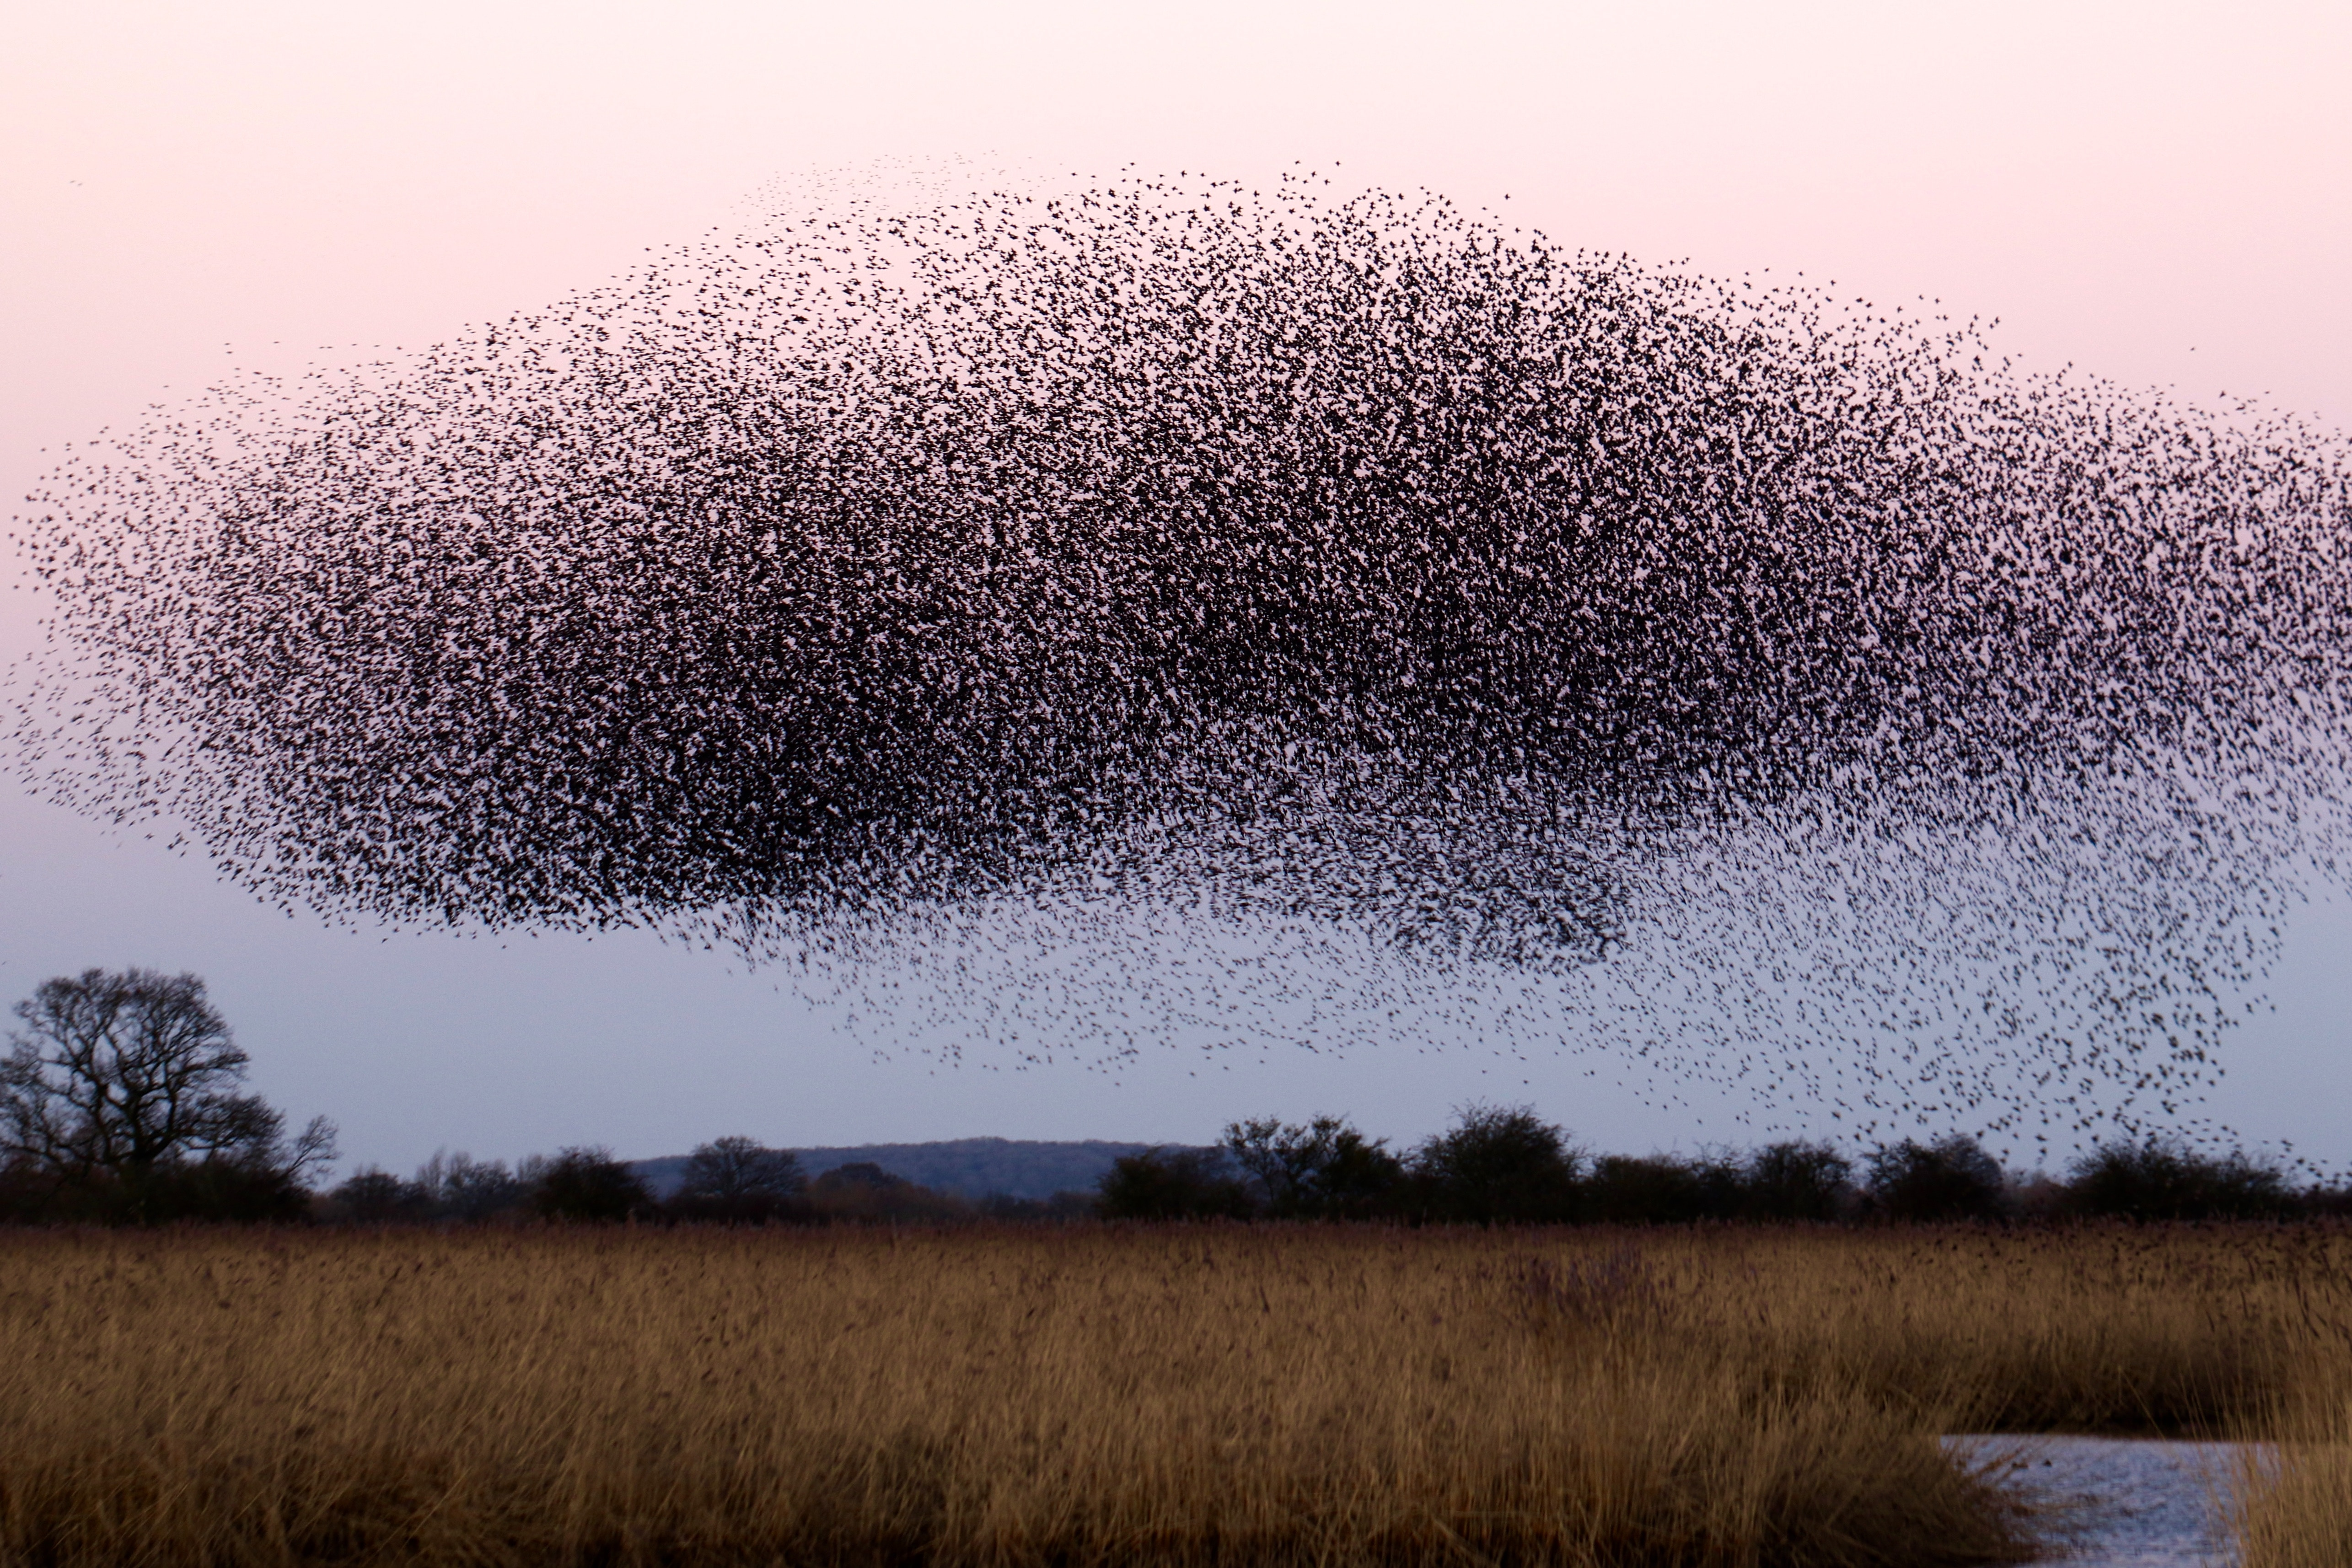
\includegraphics[width=0.9\linewidth]{images/james-wainscoat-swarm.jpg}}

	\caption{
		A classic example of swarming starlings.\cite{jameswainscoatphoto}
		In this case the swarm has coincidently taken on a shape resembling a whale.
	}

	\label{fig:birdswarm}
\end{figure}

\section{\label{sec:level1}Standard Behaviours}
A large proportion of behaviour may be interpreted logicaly, through the base instincts of fear and the requirement of social interaction.
The heavy emphasis of social interaction is a result of years of evolution requiring the animals to seek safety in numbers against their predators.
The various theories behind swarming range from from complex ``group minds"\cite{diffusionadaption} to the significantly simplified set of rules which govern what is effectively a stochastic model.\cite{modellingflocks}
These simplified behaviours were classicaly modeled in 1986 with a program named ``Boids"\cite{boids} to great success.
This program provides a set of rules to allow the simple simulation of swarming animals.

\subsection{\label{sec:level2}Reaction to a predator}

\begin{figure}[!htp]
	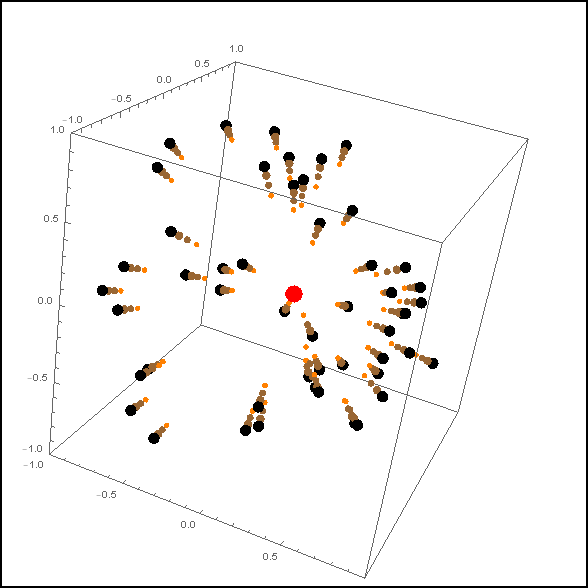
\includegraphics[width=0.7\linewidth]{images/predator.png}

	\caption{
		Several animals (in black) fly from a predator (in red).
		The velocity at which the creature attempts to escape is greatly affected by the distance to the predator.
	}

	\label{fig:animalpredator}
\end{figure}

The most drastic change to swarm behaviour occurs when a predator, lapse in cohesion or any other danger to the swarm occurs.
The natural instinct for any swarm-capable animal when faced with immediate danger is to quickly remove itself from the general path of said danger.
This results in a swarm reacting and possibly collapsing in one of the following scenarios:
\begin{description}
	\item{An individual leaves the swarm -} The tamest scenario for the swarm, one individual is forced out and made vulnerable but the swarm retains integrity.
	\item{The swarm splits -} If there is a large enough disturbance, but the alignment of most animals remains in synch, the swarm may split into seperate smaller swarms which may re-merge at a later time.
	\item{Chaotic collapse -} If the alignment of the swarm is challenged (i.e. a sufficiently large group within the swarm rapidly changes direction) then the swarm may rapidly expand in a chain reaction and lose the majority of is protective properties (FIG. \ref{fig:animalpredator}), requiring a complete reorganisation.
\end{description}

\subsection{\label{sec:level2}Reaction to a friend}

\begin{figure}[!htp]
		\fbox{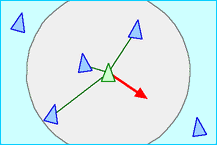
\includegraphics[width=0.45\linewidth]{images/separation.png}}
		\label{fig:boidseparation}
		\fbox{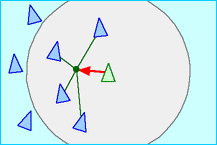
\includegraphics[width=0.45\linewidth]{images/cohesion.png}}
		\label{fig:boidcohesion}
		\fbox{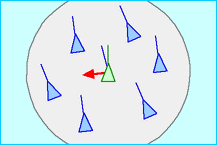
\includegraphics[width=0.45\linewidth]{images/alignment.png}}
		\label{fig:boidalignment}

	\caption{The main principles of direct flock interaction: Separation, Cohesion, Alignment.\cite{boids}}

	\label{fig:flockinteraction}
\end{figure}

The integrity of a swarm relies on the individual animals being aware of their surroundings, speed and direction.
This is almost entirely governed by neighbouring animals in a swarm.
This is one of the sticking points in a model not based on OOP principles.
Each animal, or represented point has to act indepedently of the other points and calculation complexity increases to the power of points simulated.
To maintain stability, each animal in a swarm must maintain some distance from the animals surrounding it.
The animals however must be as closely packed as possible.
To ensure these rules are met, the creatures tend to  align itself in a similar way to its neighbours.
These calculations must be carried out for each animal and in relation to every other animal.

\begin{description}
		\item{Separation - Finding the space to move in the swarm.}
		\item{Cohesion - Bringing the swarm together.}
		\item{Alignment - Allowing the swarm to stay together.}
\end{description}

\subsection{\label{sec:level2}Reaction to a goal/leader}

\begin{figure}[!htp]
	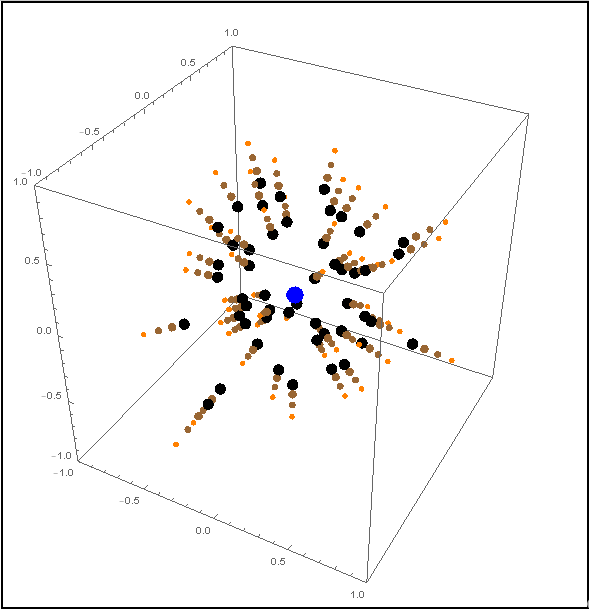
\includegraphics[width=0.3\textwidth]{images/leader.png}

	\caption{
		Several animals (in black) fly towards a goal (in blue).
		The velocity at which the creature attempts to reach the goal is affected positively by distance.
	}

	\label{fig:boidleader}
\end{figure}

To generally control the swarm, a target (for example a food source) must be utilised in the model.
In the simplest case this may be the centre of the screen (0,0).
It may also be a moveable point, possibly representing a desired direction or leader, although studies have shown that swarming lacks a definite leader in almost all cases.\cite{modellingflocks}
The draw to the leader is programatically defined to be directly proportional to the distance from the target. (FIG. \ref{fig:boidleader})

\subsection{\label{sec:level2}Combined behaviour of birds and fish}
As mentioned previously, animals swarm for the purpose of safety. Birds and fish are particularly a good example of this with both having different reasons and protection mechanisms that enable this.??\\
\indent Birds have extremely keen eyesight and therefore hiding in large numbers does not work. However, due to the effects of gravity, avivores must actively engage in flight motion, which requires the target to have enough space around it, and so they are forced to hunt birds that are at the edge of the flock, to avoid collision, which in turn incetivises cohesion among flocking birds.\\
\indent Bird flocking is a relatively simple behaviour that does not have any specific shape or form, disregarding a flock a of migratory birds. Their defence against predator is also quite primitive but actually very simple. When attacked, the birds simply disperse into all directions. This is effective because the actual predator has to avoid collision as well and therefore has to be extremely mindful of what it is attacking and focus only at the edges of the flock.\\
\indent Conversely, fish group because the aquatic environment scatters and absorbs light, which gives the fish somewhat of a cover and therefore as the predator randomly searches the environment, they are less likely to find the fish. However, the fish must also have a mechanism of how to avoid being eaten. As mentioned previously, fish need to have a mechanism to avoid being eaten when faced with a predator. Schools have adopted the so called fountain manoeuvre, which takes advantage of the predator's momentum by swimming towards it when it attacks. 

\begin{figure}[!htp]
	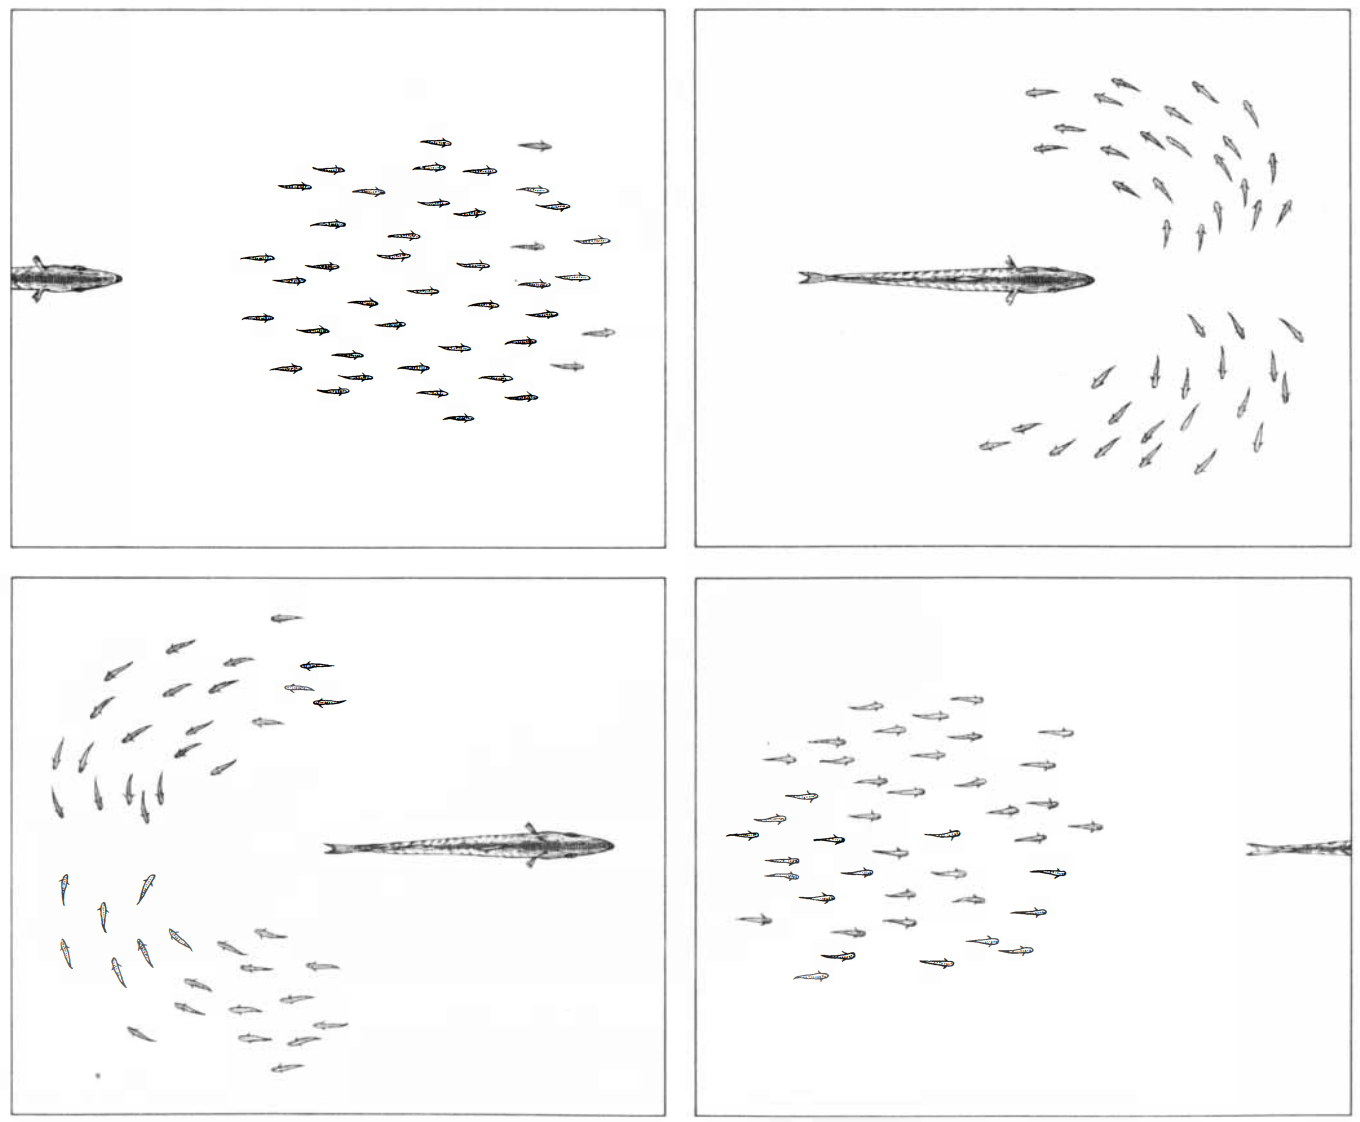
\includegraphics[width=0.48\textwidth]{images/partridgeFountain.png}

	\caption{
		Fountain movement made by the fish.
	}

	\label{fig:boidleader}
\end{figure}

Finally, the information that is carried through the swarm starts out slowly but eventually increases to large speeds. This has been observed to be somewhat exponential. %Move this somewhere else?

\section{\label{sec:level1}Object Oriented Programming (OOP)}

Mathematica does not inherently support object oriented programming, so the majority of the calculations for larger swarms mjust be solved using matrices.
The crux of the matter is that the swarm, leader and predator all behave differently, and so must be programmed as separately as possible.
The 3 differently behaving types should also be able to interact, obtaining data from each others positional matrices.

\subsection{\label{sec:level2}Heavy OOP method}

The first attempted solution involved the strict separation of:
\begin{description}
	\item{Swarming Animals - Known as boids.}
	\item{Leader - To allow a target point, or food source.}
	\item{Predator - To disturb the group of boids.}
\end{description}

These individual "Objects" were programmed in the following ways:
\begin{enumerate}
	\item{
		The boids were programmed to randomly choose another boid to follow, and a boid to avoid.
		Each calculation round would haved the boid move towards the followed boid based on the euclidean distance and away from the avoided boid based on inverse euclidean distance.
 }
 	\item{
		The leader and predator were programmed to follow intersecting paths to simulate the collision of the hunter and the swarm.
		In both cases the speed was normalised to be independent of movement path diameter.
	}
\end{enumerate}

The program initialy assigns the boids to a random point on a map of fixed size.
In each calculation stage, a unit vector, representing the direction of the leader to the boid is calculated.
This unit vector is multiplied by a scalar value corresponding to a fraction of the distance between the boid and the leader.
The resulting vector is added to each boids current position.

A nearly identical process occurs for the enemy, however it moves the boid away from the predator.
The scalar value also increases with the decrease in euclidean distance, resulting in a large reaction should the predator be nearby.

To calculate the movement between boids, a matrix containing a list of followers calculates a new matrix based on the distance between each boid and the boid it is following.
This vector distance is then divided by a scalar value and added to each boid.
The same process occurs in reverse for each boids enemy.

\begin{figure}[!htp]
	\fbox{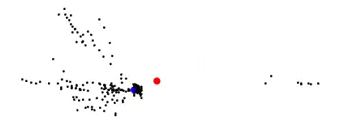
\includegraphics[width=0.7\linewidth]{images/lines.png}}

	\caption{
		Several animals form lines around the leader.
		The predator has succeeded in separating a group from the main swarm.
	}

	\label{fig:animallines}
\end{figure}

The working code is shown in \href{https://youtu.be/EyhdRhi5Gnc}{2D Video} and \href{https://youtu.be/KG7qQum6EUc}{3D Video} formats.


\subsection{\label{sec:level2}Light OOP method}

It was decided that a swarm did not inherently require a moveable target and instead should simply attempt to retain integrity.
It is thought that of the 20,000+ known species of fish, half will at some point in there lives form a school.\cite{fishschools}
This led to the development of a second model, loosely based on the first.
The behaviour of the predator was also improved to instead pick a specific boid and hunt it down.
The interactions also allow the predator to ``eat" the boid, removing it from the swarm.

One of the most distinctive properties of an underwater swarm is its use in evading enemies.
This is due to the ``blindness" of the predator and predated fish in murky waters.
The maximum theoretical distance visible underwater is 80 m, and the furthest observed in calm, clear water is 74 m.\cite{underwatervision}
By forming a tight swarm, the predator has a significantly reduced chance of randomly finding the fish than if they were spread throughout an area. (FIG. \ref{fig:swarmblindness})

\begin{figure}[!htp]
		\fbox{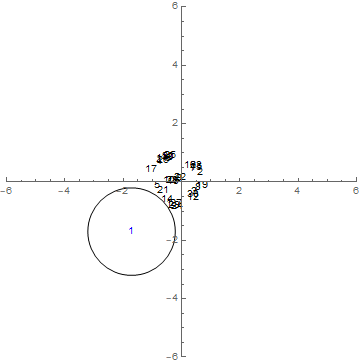
\includegraphics[width=0.465\linewidth]{images/hunterCircleBefore.png}}
		\label{fig:swarming}
		\fbox{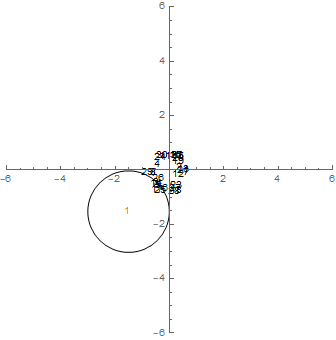
\includegraphics[width=0.465\linewidth]{images/hunterCircleAfter.png}}
		\label{fig:noswarming}
		
	\caption{The effects of swarming mitigating the ability (represented by the black circle) of the hunter to detect the fish.\cite{underwatervision}}

	\label{fig:swarmblindness}
\end{figure}

To keep the boids on screen, a slight move towards the center of the model each calculation roud was added.
Other vector components included were random noise and a move towards the center of the group of boids around the boid being calculated.
It was decided to use a logarithmic weighting for these calculations, where the closest boid represented the largest influence and a calculation for these weightings was calculated as a constant array, allowing quick application and the ability of the model to run in real time.
To gain data on the effectiveness of this swarming and hiding, a ``kill" function was added to the hunter, where boids within a certain distance of the hunter would be eaten, and the data for this function recorded for each calculation step, resulting in a plot of living boids with time.

\section{\label{sec:level2}Discussion}
Light OOP was chosen
Post death rate and compare between 2D and 3D %in images under popDec
Point out the oribiting problem %an image should exist as well

\section{\label{sec:level1}Conclusion}
Theory was discussed
Different approached were discussed
Light OOP method was chosen because of use with the Mathematica tool
The performance of the model was fairly good as the death rate is not constant
There's also the fact that the boids stick to the origin for better testing
Also, in 2D, boids form donuts but this is okay as the model we have is designed for 3D, not 2D.

Mention that it would be more interesting to work on hunters


% ****** Past here be the bibliography ******

	\bibliographystyle{ieeetr}
	\bibliography{references}

\end{document}

% ****** End of file main.tex ******
